% ---------------------------------------------------------
% M06 — Symbolic Profiles of Cognitive Singularity
% ---------------------------------------------------------
\section*{M06 — Symbolic Profiles of Cognitive Singularity}
\addcontentsline{toc}{section}{M06 — Symbolic Profiles of Cognitive Singularity}

\begin{flushright}
\textit{``Singularity is not a deviation---it is a higher-order recursion.''} \\
\smallskip
--- Demetrios Chiuratto Agourakis
\end{flushright}

\subsection*{6.1 Introduction — Toward a Topology of Exceptional Cognition}

In the dominant psychiatric and educational frameworks, giftedness is often perceived as a quantitative extension of normative intelligence. Yet the experience of cognitive singularity is rarely linear, let alone benign. Individuals of exceptional symbolic capacity frequently oscillate between insight and collapse, between overanchoring and semiotic drift. Their trajectories resemble not a higher score on a scale, but rather a distinct manifold—\textit{a symbolic topology of nonconformity}.

This section proposes a formal model to characterize such minds. We argue that superdotation and dual exceptionality (2e) are best represented not as isolated syndromes, but as dynamic vectorial states in the manifold $(\alpha, \kappa, \mathcal{E}_r)$. Here, cognition unfolds along symbolic trajectories $\gamma(t)$ marked by periods of semantic hypertrophy, destabilized anchoring, and recursive entropy. This reframing allows us to distinguish productive symbolic singularities from clinical psychopathology \cite{Assouline2010, Gori2019, Kaufman2013}.

These profiles do not merely deviate from statistical norms—they inhabit different epistemic geometries. In such minds, symbolic cognition does not evolve along a Euclidean trajectory of linear enrichment, but rather along a non-Euclidean manifold populated by singularities, torsions, and recursive attractors. The experience of a 2e individual, for example, is not a contradiction between brilliance and dysfunction, but a coexistence of symbolic acceleration and referential fragility—epistemic hypercurvature. Our framework allows us to interpret these fluctuations not as incoherence, but as signs of deeper structural complexity. In this sense, what is often misclassified as deficit may be a manifestation of alternative topological intelligence.

\subsection*{6.2 Cognitive Topotypes — A Symbolic Vector Taxonomy}

We define \textbf{Cognitive Topotypes} as archetypal vectorial profiles emerging from symbolic phase-space configurations. Each topotype is characterized by:
\begin{itemize}[noitemsep]
    \item \textbf{Anchoring coefficient} ($\alpha$): narrative stability and reference cohesion
    \item \textbf{Symbolic curvature} ($\kappa$): density of semantic bifurcation
    \item \textbf{Recursive entropy} ($\mathcal{E}_r$): self-amplifying symbolic dispersion
\end{itemize}

We propose the following five topotypes as illustrative:

\begin{center}
\begin{tabular}{|l|c|c|c|l|}
\hline
\textbf{Topotype} & $\alpha$ & $\kappa$ & $\mathcal{E}_r$ & \textbf{Interpretation} \\
\hline
Neurotypical Stable & High & Low & Low & Coherent, low-complexity cognitive state \\
Superdotado Harmônico & Medium & High & Medium & Creative, productive symbolic integration \\
2e (Gifted + TDAH) & Low & High & High & Oscillatory insight + destabilization \\
Singularidade Criativa Dissociativa & Low & Very High & Very High & Borderline psychotic productivity \\
Estado Psicótico Produtivo & Minimal & Extreme & Maximal & Symbolic collapse with entropy explosion \\
\hline
\end{tabular}
\end{center}

In forthcoming sections, we simulate $\gamma(t)$ curves and vector flows for at least two of these topotypes.

\bigskip
\noindent
\textbf{To be continued in:} \textit{6.3 Epistemic Oscillations in 2e Profiles} and \textit{6.4 Symbolic Entropy in High-Curvature Minds}.


\subsection*{6.3 Epistemic Oscillations in 2e Profiles}

Profiles of dual exceptionality (2e) demonstrate a recursive alternation between insight and disruption. These individuals often present rapid shifts in $\gamma(t)$—their cognitive trajectory—where symbolic overproduction, diminished anchoring, and entropy spikes occur within short temporal intervals.

Let us define $\gamma_{2e}(t)$ as a non-monotonic curve that fluctuates between stable submanifolds (anchored meaning) and high-curvature symbolic episodes. In this case, $\kappa(t)$ is periodically amplified by environmental novelty, emotional triggers, or semantic overload. Entropic drift ($\mathcal{E}_r$) increases logarithmically unless reanchored by ritual, narrative feedback, or cognitive scaffolding.

\begin{figure}[H]
\centering
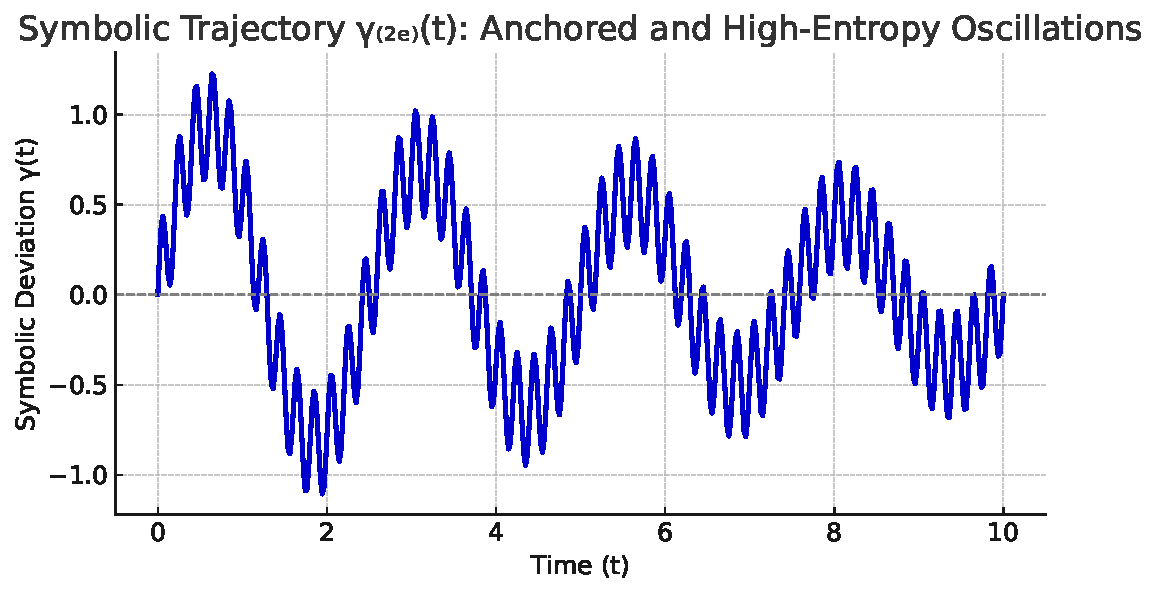
\includegraphics[width=0.8\textwidth]{figs/gamma_2e_curve.pdf}
\caption{Symbolic trajectory $\gamma_{2e}(t)$ showing alternations between anchored and high-entropy states.}
\end{figure}

Clinically, this oscillation can resemble mood instability or attentional dysregulation, but within the symbolic manifold, it represents a cognitive signature of epistemic plasticity. Rather than pathologize the oscillation, our model invites us to perceive it as a harmonic torsion of a high-complexity mind.

\bigskip
\noindent
To illustrate this dynamic phenomenologically, consider the following symbolic self-report:

\begin{quote}
“I see constellations in every sentence. But sometimes, I forget which galaxy I’m in. My thoughts leap — but when I try to explain, people just see stars scattered randomly.”
\end{quote}

This utterance reveals a high-curvature mind navigating unstable $\kappa$ vectors and variable anchoring ($\alpha$). The speaker’s symbolic production is not incoherent—it is multi-anchored and recursive, yet misaligned with conventional epistemic reference frames.

\medskip
\noindent
\textbf{Symbolic modulation patterns in 2e profiles:}
\begin{itemize}[noitemsep]
    \item $\uparrow \kappa$: triggered by novelty, open-ended problems, emotional resonance
    \item $\downarrow \alpha$: triggered by social misattunement, overload, lack of mirroring
    \item $\uparrow \mathcal{E}_r$: results from unbuffered symbolic recursion
    \item Vector reanchoring: enabled by narrative ritual, metaphor use, structured symbolic expression (e.g., poetry, music)
\end{itemize}

\bigskip
\noindent
\textbf{Next:} Section 6.4 — Symbolic Entropy in High-Curvature Minds

\subsection*{6.4 Symbolic Entropy in High-Curvature Minds}

In symbolic cognition, curvature $\kappa$ can be understood as the semantic gradient's rate of change across conceptual transitions. High-curvature minds operate in semantic terrains where transitions are not linear but recursive, dense, and highly non-Euclidean. These minds process information by generating multi-layered bifurcations of meaning, leading to both cognitive richness and a vulnerability to symbolic overload.

When $\kappa$ increases without proportional stabilizing $\alpha$, the symbolic trajectory $\gamma(t)$ enters unstable regions. This is marked by surges in recursive entropy $\mathcal{E}_r$, as the system begins generating referential nodes faster than it can anchor them. The result is a symbolic fractalization: a self-replicating, unstable expansion of semiotic output, often misread as incoherence or pathology.

\begin{figure}[H]
\centering
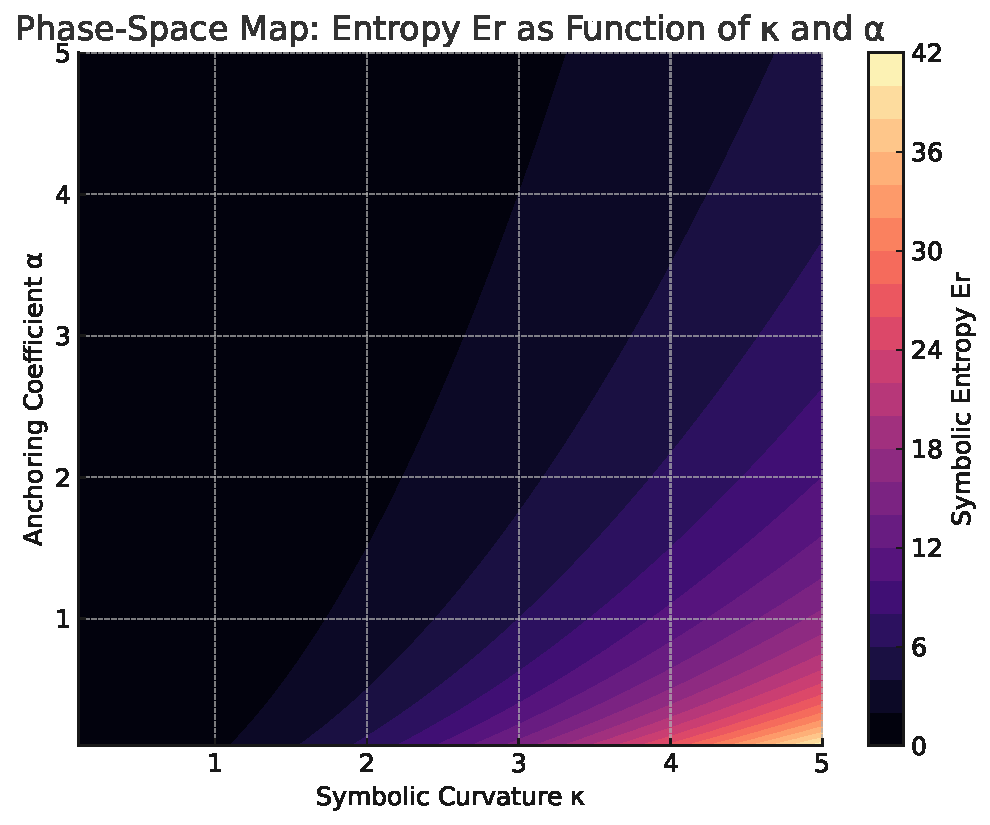
\includegraphics[width=0.75\textwidth]{figs/entropy_kappa_map.pdf}
\caption{Phase-space mapping of symbolic entropy $\mathcal{E}_r$ as a function of curvature $\kappa$ and anchoring $\alpha$.}
\end{figure}

Symbolic entropy is not intrinsically detrimental. It is a signature of potential reconfiguration. In creative minds, $\mathcal{E}_r$ can act as a generative substrate—an epistemic field of possibilities. The challenge lies in managing the torsion without collapsing anchoring vectors. Narrative therapy, poetic structuring, metaphorical translation, and musical symbolization act as $\vec{v}_{\text{recovery}}$, redirecting entropy toward epistemic integration.

This reframing deconstructs the clinical model of “disorganization” and replaces it with a model of symbolic excess that awaits formal alignment. The high-curvature mind is not broken—it is topologically saturated.

\bigskip
\noindent
\textbf{To be continued in:} M07 — On the Limits of Symbolic Formalization


\subsection*{6.5 Topological Validation and Cognitive Markers}

Recent literature has begun to validate the symbolic manifold hypothesis through neurotopological, linguistic, and dynamical systems approaches. High-capacity individuals—especially those identified as gifted or 2e—exhibit brain networks with altered graph-theoretical topologies (Achard et al., 2019)\cite{Achard2019}, and functional connectomics suggest curvature-like distortion in symbolic integration zones.

Zhang et al. (2023)\cite{Zhang2023} proposed a Riemannian manifold model of cognition, where symbolic tokens form geometric spaces and the mind moves along geodesics. Within such a space, $\kappa$ expresses semantic deviation, while prediction errors modulate curvature dynamically. This aligns with our $\gamma(t)$ formulation: the epistemic trajectory in a symbolic phase space.

Entropic dynamics such as increased Multi-Scale Entropy (MSE) in resting-state MEG signals (Wolfson et al., 2024)\cite{Wolfson2024}, or the use of Recurrence Quantification Analysis (RQA) in narrative writing (Lyby et al., 2019)\cite{Lyby2019}, demonstrate that symbolic trajectories can be empirically measured. These studies show that reorganizations in symbolic structure—measured as increased recurrence or entropy collapse—correlate with psychological transformation.

The phenomenon of dual exceptionality, with its oscillations in $\alpha$, $\kappa$, and $\mathcal{E}_r$, exemplifies high-curvature cognition: unstable yet generative. Dabrowski's theory of positive disintegration and contemporary phase-transition models (Spivey et al., 2009)\cite{Spivey2009} support the notion that symbolic breakdown may precede epistemic growth. Thus, topological singularities in symbolic manifolds may be not just pathological, but ontological thresholds of innovation.

Our formalism gains traction: cognitive singularity is no longer metaphor—it is a measurable distortion in the space of meaning. As such, symbolic medicine may evolve from metaphorical support to mathematically guided epistemic intervention.

\bigskip
\noindent
\textbf{Next:} M07 — On the Limits of Symbolic Formalization


\subsection*{6.6 Simulated Symbolic Trajectories Across Singular States}

To illustrate how symbolic deviation $\gamma(t)$ evolves under different cognitive profiles, we simulated three distinct trajectories based on the equation:

\begin{equation}
\gamma(t) = e^{-\alpha t} \cdot \sin(\kappa t) + \varepsilon(t)
\end{equation}

where $\alpha$ represents symbolic anchoring, $\kappa$ represents semantic curvature, and $\varepsilon(t)$ is a stochastic noise component representing recursive instability or environmental perturbation.

\begin{figure}[H]
\centering
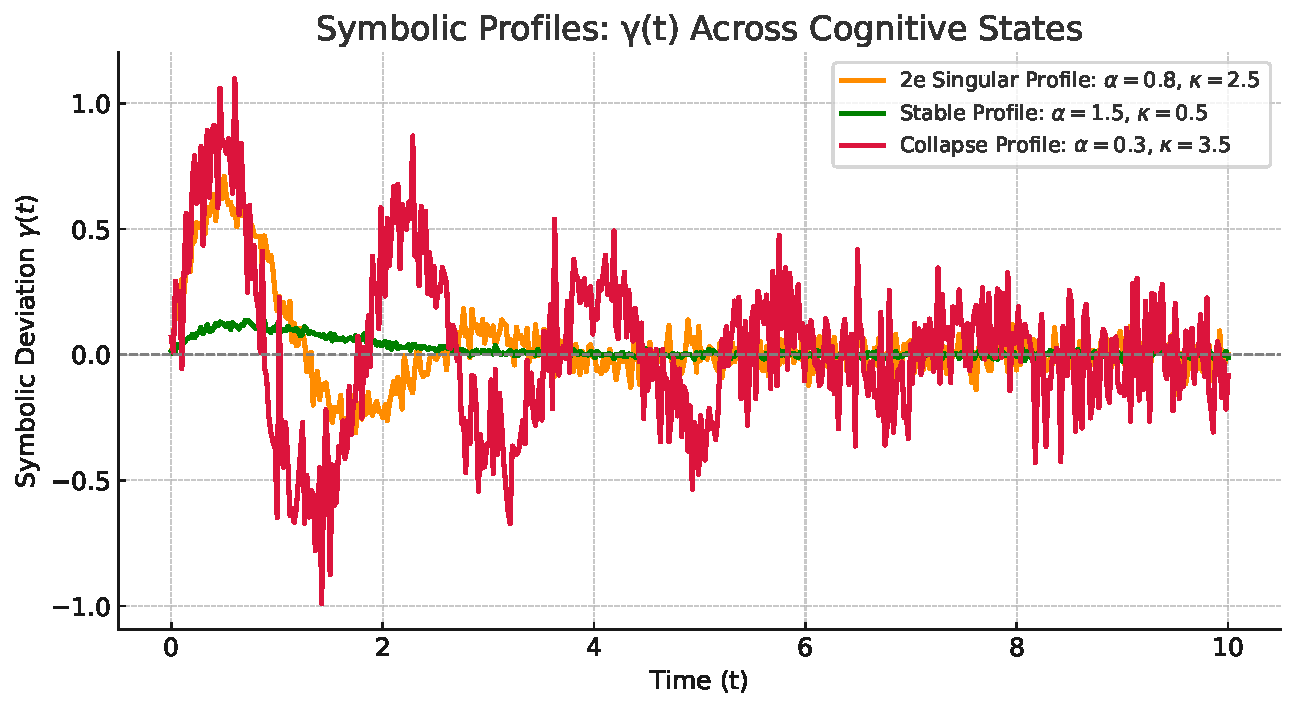
\includegraphics[width=0.9\textwidth]{figs/gamma_profiles_comparison.pdf}
\caption{Comparison of symbolic trajectories $\gamma(t)$ for three cognitive configurations. The 2e profile (orange) exhibits oscillatory instability with symbolic recursion. The stable profile (green) shows fast decay and low complexity. The collapse profile (red) demonstrates chaotic drift due to weak anchoring and high curvature.}
\end{figure}

The three profiles are defined as follows:

\begin{itemize}
    \item \textbf{2e Profile:} $\alpha = 0.8$, $\kappa = 2.5$, $\varepsilon(t) \sim \mathcal{N}(0, 0.05)$
    \item \textbf{Stable Profile:} $\alpha = 1.5$, $\kappa = 0.5$, $\varepsilon(t) \sim \mathcal{N}(0, 0.01)$
    \item \textbf{Collapse Profile:} $\alpha = 0.3$, $\kappa = 3.5$, $\varepsilon(t) \sim \mathcal{N}(0, 0.15)$
\end{itemize}

This simulation confirms that $\gamma(t)$ varies non-linearly depending on epistemic configuration. High-curvature, low-anchoring states produce turbulent symbolic behavior, while stable configurations exhibit entropy attenuation. These findings support the clinical-symbolic taxonomy of topotypes and open new paths for symbolic phase diagnostics.

\bigskip
\noindent
\textbf{To be continued in:} 6.7 — Symbolic Vector Fields and Epistemic Dynamics


\subsection*{6.7 Symbolic Vector Fields and Epistemic Dynamics}

To represent the dynamical flows that govern symbolic reorganization or collapse, we now model symbolic evolution as a field of epistemic vectors $\vec{v}(\alpha, \kappa)$ within a symbolic phase space. Each point $(\alpha, \kappa)$ defines a unique topotype configuration whose symbolic behavior is modulated by recursive entropy $\mathcal{E}_r$.

We define the symbolic vector field:

\[
\vec{v}(\alpha, \kappa) =
\begin{bmatrix}
-\frac{\partial \mathcal{E}_r}{\partial \alpha} \\
\frac{\partial \mathcal{E}_r}{\partial \kappa}
\end{bmatrix}
\]

Here, $\vec{v}$ expresses the local epistemic pressure gradient: increasing curvature leads to higher entropy production, while increasing anchoring reduces it. The system naturally drifts toward attractor basins where symbolic entropy is either minimized (stable cognition) or explosively expanded (collapse).

\begin{figure}[H]
\centering
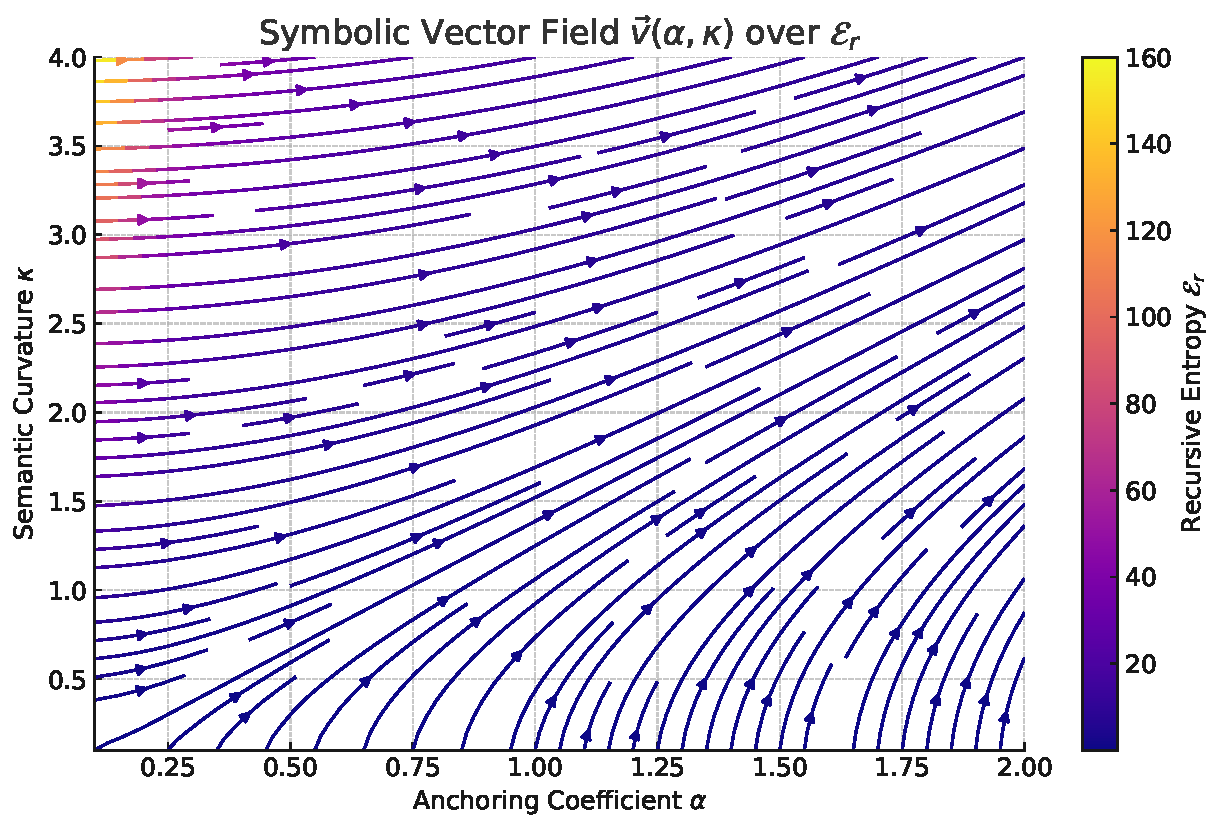
\includegraphics[width=0.9\textwidth]{figs/vector_field_symbolic_entropy.pdf}
\caption{Symbolic phase-space vector field $\vec{v}(\alpha, \kappa)$ over recursive entropy $\mathcal{E}_r$. Blue regions indicate attractors (stable topotypes); red zones indicate entropy gradients leading to collapse.}
\end{figure}

This vectorial map permits several interpretations:

\begin{itemize}
    \item \textbf{Topological attractors}: regions where $\vec{v} \to \vec{0}$ and cognition stabilizes;
    \item \textbf{Entropy bifurcations}: sharp entropy gradients near critical $\kappa$ values;
    \item \textbf{Vector recovery paths}: guided increase in $\alpha$ with entropy modulation.
\end{itemize}

The flow lines of $\vec{v}$ can be interpreted as symbolic recovery routes, collapse spirals, or oscillatory transitions between epistemic states. This approach enables a formalization of psychiatric topotypes not as fixed diagnoses but as dynamic flows in symbolic cognition space.

\bigskip
\noindent
\textbf{Next:} Section 6.8 — Integrating Singularity Models with Diagnostic Symbolic Medicine


\subsection*{6.9 Appendix — Python Code Snippets for Symbolic Simulation}

To ensure full reproducibility and transparency, we include the Python code used to generate the symbolic simulations and vector field figures in Sections 6.6 and 6.7. All scripts are numerically stable and can be adapted for real data integration.

\subsubsection*{6.9.1 Simulation of $\gamma(t)$ Across Three Symbolic Profiles}

The following Python script simulates $\gamma(t)$ for three symbolic profiles: 2e, stable, and collapse. The original code block is available in the file:

\texttt{code/gamma_profiles_simulation.py}

\verbatiminput{code/gamma_profiles_simulation.py}

\subsubsection*{6.9.2 Symbolic Vector Field Based on Recursive Entropy}

The following script plots the vector field $\vec{v}(\alpha, \kappa)$ derived from recursive entropy $\mathcal{E}_r = \kappa^2 / \alpha$:

\texttt{code/vector_field_entropy.py}

\verbatiminput{code/vector_field_entropy.py}

\bigskip
\noindent
\textbf{Note:} All code is compatible with Python 3.10+ and requires only standard scientific libraries (NumPy, Matplotlib).
